\documentclass{article}
\usepackage{tikz}
\usepackage[top=2cm,bottom=2cm,right=2cm,left=2cm,a4paper]{geometry}

\begin{document}
\pagestyle{empty}
\noindent
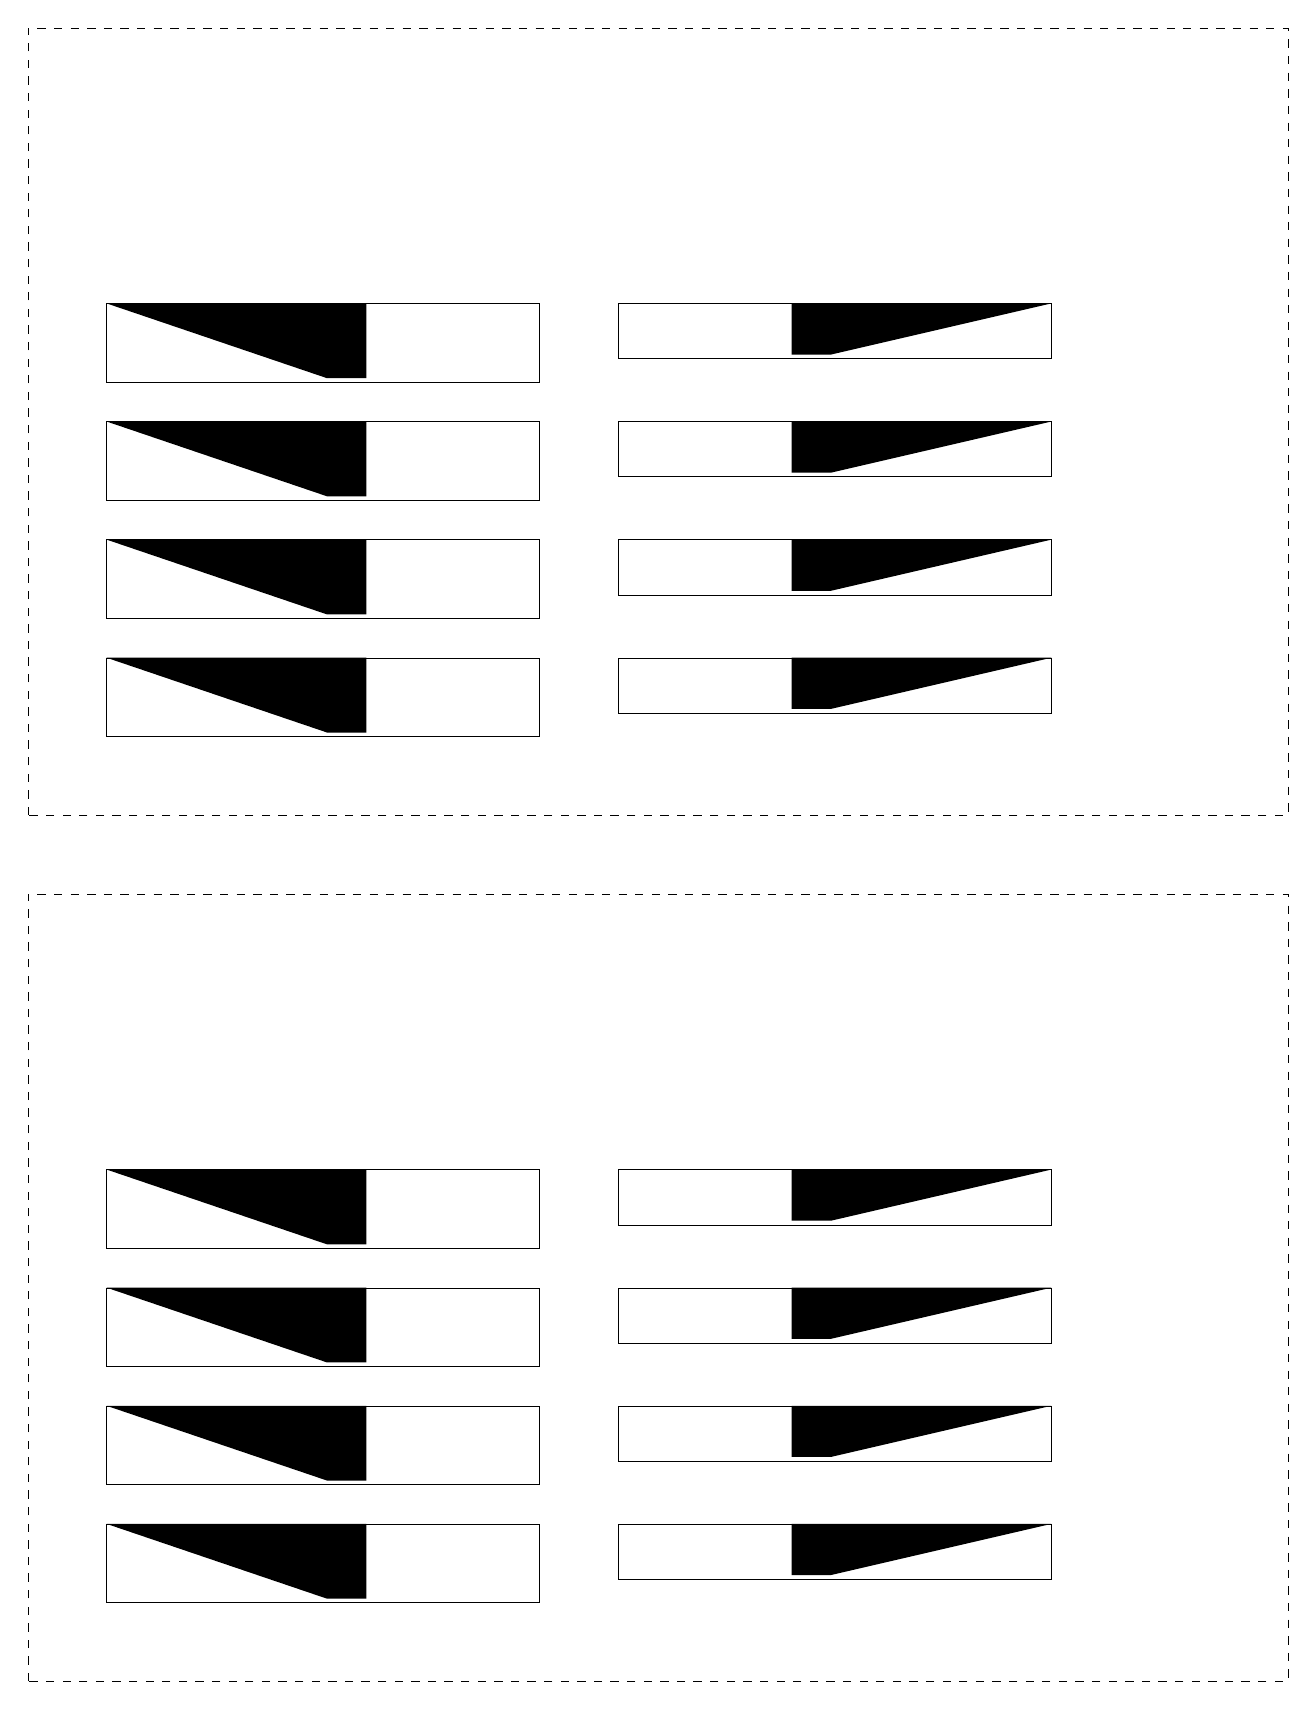
\begin{tikzpicture}[ultra thin]
    % \draw[help lines,step=10mm,black!20,thick] (-0mm,-10mm) grid (140mm,40mm);
    % \draw[help lines,step=1mm,black!20] (-0mm,-10mm) grid (140mm,40mm);


    \foreach \x in {0mm, 110mm} {
        \begin{scope}[yshift=\x]
            \draw[dashed] (0,0) rectangle (160mm, 100mm);
            \foreach \y in {0mm, 15mm, 30mm, 45mm} {
                \begin{scope}[yshift=\y+10mm, xshift=10mm]
                    \begin{scope}
                        \draw (0mm,0mm) rectangle (55mm, 10mm);
                        \path[fill=black] (28mm,0.5mm) -- ++(right:5mm) -- 
                        ++(up:9.5mm) -- ++(left:5mm) 
                        -- (0mm,10mm) -- cycle;
                    \end{scope}

                    \begin{scope}[yshift=3mm, xshift=55mm+10mm]
                        \draw (0mm,0mm) rectangle (55mm, 7mm);
                        \path[fill=black] (27mm,0.5mm) -- ++(left:5mm) -- 
                        ++(up:6.5mm) -- ++(right:5mm) 
                        -- (55mm,7mm) -- cycle;
                    \end{scope}
                \end{scope}
            }
        \end{scope}
    }
\end{tikzpicture}

\end{document}
